
%(BEGIN_QUESTION)
% Copyright 2006, Tony R. Kuphaldt, released under the Creative Commons Attribution License (v 1.0)
% This means you may do almost anything with this work of mine, so long as you give me proper credit

Given the liquid flowmeter and storage vessel shown here, determine the accumulated volume in the vessel at the following times, for the flow rates shown on the graph:

$$\includegraphics[width=15.5cm]{i01581x01.eps}$$

\begin{itemize}
\item{}Time = 0:15; Volume = \underbar{\hskip 50pt}
\vskip 5pt
\item{}Time = 1:30; Volume = \underbar{\hskip 50pt}
\vskip 5pt
\item{}Time = 1:45; Volume = \underbar{\hskip 50pt}
\vskip 5pt
\item{}Time = 2:45; Volume = \underbar{\hskip 50pt}
\end{itemize} 
 
As indicated on the graph, the vessel holds 55 gallons of liquid at time = 0:00.  Note that the unit of time for the graph's horizontal axis is minutes:seconds, not hours:minutes.

\vskip 10pt

Also, calculate the accumulated volume in the liquid storage vessel at time = 1:00 and time = 2:30.  Use this information to sketch a plot of accumulated liquid volume over time.

\vskip 20pt \vbox{\hrule \hbox{\strut \vrule{} {\bf Suggestions for Socratic discussion} \vrule} \hrule}

\begin{itemize}
\item{} If you were standing in view of the pipe discharging water into this vessel, what would the liquid flow rate shown by the graph {\it look} like?  Would the flow vary over time, or would it remain steady?  Would it start and stop, or be continuous?
\item{} Suppose you were given a graph of water volume in the tank, and asked to calculate flow rate in or out of the tank.  What principle of calculus would you apply to solve this problem?
\item{} Suppose the flow rate ($Q$) shown on the graph represented flow {\it out} of the tank rather than flow {\it in} to the tank.  How would this difference affect the shape of the $V$ graph?
\item{} A tank being filled with water is analogous to an electrical capacitor being ``filled'' with charge.  Identify the appropriate variables for a graph showing the ``filling'' of a capacitor.
\end{itemize}

\underbar{file i01581}
%(END_QUESTION)





%(BEGIN_ANSWER)

\begin{itemize}
\item{}Time = 0:15; Volume = 55 gallons
\item{}Time = 1:30; Volume = 70 gallons
\item{}Time = 1:45; Volume = 70 gallons
\item{}Time = 2:45; Volume = 75 gallons
\end{itemize} 

\begin{itemize}
\item{}Time = 1:00; Volume = 58.75 gallons
\item{}Time = 2:30; Volume = 73.75 gallons
\end{itemize} 

$$\includegraphics[width=15.5cm]{i01581x02.eps}$$

%(END_ANSWER)





%(BEGIN_NOTES)





\vskip 20pt \vbox{\hrule \hbox{\strut \vrule{} {\bf Suggestions for Socratic discussion} \vrule} \hrule}

\begin{itemize}
\item{} Propose a different flow trend recording to students (e.g. different shape of trend profile) and have them predict the resulting alteration of the volume trend.
\item{} Propose a different volume trend recording to students (e.g. different shape of trend profile) and have them predict the necessary flow trend profile to cause it.
\end{itemize}


%INDEX% Mathematics, calculus: integral (accumulated volume as the integral of flow)

%(END_NOTES)


